\section{Background and Related Work}
\label{sec:background}
% subsections are \subsection{title}
%% subssubsections are \subsubsection{title}
%% numbering will work automatically 

\subsection{The history of Polish (19\textsuperscript{th}-century)}
\label{subsec:history-pl}

When discussing a historical variant of a language it is important to situate it in the context of what is known about the history of that language in general. Historical grammar and descriptions are available for many of the major languages, and Polish is no exception - although recently concerns have been raised that the some of the most thorough descriptions of the history of Polish may be outdated given more recent research, and therefore in need of being updated \citep{dunaj_19}. Nevertheless, much of the general information from these sources remains relevant, and can be supported by more recent books.

In what is considered to be one of the core texts of the study of historical Polish, \citet{klemensiewicz_76} describes the developement of that language from mid-12\textsuperscript{th} century. He characterizes it as an Indoeuropean language, and, more specifically, one belonging to the West Slavic language family. Throughout the book, the author adopts the following periodization of the language\footnote{This periodization appears to be motivated by historical events such as the turnung point between Middle Ages and the Renaissance (1500s), the Enlightenment and the partitioning of Poland (late 1700s), the start of the Second World War (1939).}: Old Polish (until 1500s), Middle Polish (from 1500s to 1780s), New Polish (from 1780s to 1939). \citet{długosz-kurczabowa_dubisz_2006} adopt a similar division, but they include subdivision of both the Middle Polish and New Polish periods into parts 1 and 2, introducing a more fine-grained distinction. 

While \citet{klemensiewicz_76} provides an extremely thorough characterization of each of those periods, including the socio-historical context, only the New Polish period appears to be relevant to the topic of this thesis, and therefore it is this period whose characterization will be discussed in more detail. The duration of the New Polish period is characterized by many political and social changes, including a long-term occupation by a number of various countries; nevertheless, that period of unrest was preceded by some attempts at describing the contemporaneous Polish language. Although the time of partitioning of Poland was characterized by certain repressions when it came to e.g. receiving education in Polish, the language was not pushed out of use, partly due to different areas being subject to different rules, and partly due to strong resistance and a "national spirit." Although this situation only worsened as time progressed, the author attributes the survival of the Polish language and identity, especially in East Poland, to family and traditional upbringing. It is relevant to point out that even this seemingly difficult time period featured the creation of e.g. dictionaries of Polish. 

\citet{klemensiewicz_76} characterizes the changes that were taking place in the New Polish period as the following:
\begin{enumerate}
    \item Phonology: final loss of ȧ, ė, ȯ (close versions of /a/, /ɛ/, /o/, a remnant of the long-short distinction in the Polish vowel system); reduction of /ija/ and /ɨja/ to /ja/ in borrowings; depalatalization of syllable-final soft consonants; adoption of the pronunciation /ɕr/ over /ɕʐ/ and /ʑr/, /jʐ/ over /ʑʐ/; variation in the pronunciation of sibilant sounds; establishment of modern-like stress patterns (penultimate syllable, including clitics; separate stress in the constituent words of compound phrases). 
    
    \item Inflection of nouns: continued variation in the masculine singular genitive and dative forms; adoption of the plural accusative as the plural nominative form in the masculine paradigm, with a following pejoration of these forms in some cases; loss of the -a ending for plural nominative forms Latin borrowings; gradual loss of the -ów ending in the plural genitive masculine nouns whose root ends in a soft consonant; plural genitive endings taking over plural accusative, the original endings persisting only in stylized texts; -ę replacing -ą in the majority of feminine nouns in singular accusative; variation between -e, -i, and -y as nominative, accusative, and vocative forms of plural feminine nouns; loss of the "masculine" ending -ów used in feminine and neuter plural genitive nouns; temporary loss of the nasal /ɛ̃/ in favor of /ɛ/ in nominative and accusative singular forms of neuter nouns; loss of the -y and -i endings for the plural instrumental forms of neuter and masculine nouns in favor of -ami and -mi.
    
    \item Inflection of pronouns and adjectives: gradual loss of the -ę ending in singular accusative feminine pronouns in favor of -ą; continued variation in the endings (-ym, -im, -em, -ymi, -imi) for the instrumental and locative singular masculine and neuter forms as well as the plural instrumental forms of pronouns and adjectives.
    
    \item Inflection of numerals: generalization of the -u ending in numerals; two parallel forms of the dative form of \textit{dwa} `two', replacement of -ą with -u in the instrumental case of numerals.
    
    \item Verbal inflection: replacement of -m with -my in the first person plural in the present tense; the loss of the pluperfect tense; preference for attaching of the conditional marker to the l-participle; preference for constructing the future tense by combining an auxiliary verb \textit{być} `to be' with the l-participle instead of the infinitive; development of the -szy ending of the past participel forms into -łszy or -wszy; attempts of reviving the dual forms.
    
    \item Word formation: increase of the popularity of zero-derivation; fall of the popularity of derivational suffixes such as -ak, -nik, -ły, -ec; preference for derivational suffixes -arz, -acz, -dło in narrow fields (e.g. technical, artistic); prominence of derivational suffixes -ik, -ina, -isko, -ość, -stwo, -i, -y, -ić; change of meaning of the derivational suffix -ek; prevalence or acronyms.

    \item Syntax: preference for the nominal subject complement to be in the instrumental case, while for an adjectival one to be in the nominative; replacement of the genitive by the accusative in object position; tendency to inflect \textit{jeden} `one' in double-digit numerals; preference for rection over agreement in double-digit numerals ending with \textit{dwa} `two'; decrease in popularity of the preposition \textit{ku} `towards, for, in order to'; rise in popularity of a new form of the final clause consisting of a conjunction followed by the infinitive form of the verb if the subject of both clauses is the same; loss of a variety of conjunctions and particles; variation between the pronouns \textit{co} `what, which, who' and \textit{który} `which, who'. 

    \item Lexicon: increase in specialized vocabulary; raised awareness of synonyms and near-synonyms and their usefulness; loss of a variety of words; variety of neologisms or new derived words; largely negative attitudes to foreign borrowings, although those are numerous (including borrowings from Latin, French, German, Russian, Ruthenian, English.

    \item Orthography and orthophony: multiple attempts at standardization, one reform made in 1918; little adherence to normalized spelling in the press and other sources; final reform of the period in 1936; attempts at normalizing pronunciation in early 1900s.
\end{enumerate}

Other sources, such as \citet{długosz-kurczabowa_dubisz_2006} opt for separate descriptions of the evolution of different aspects of the language; nevertheless, they do provide summaries of changes happening at certain points in time. They divide the New Polish period into two parts, with the breaking point between the two around 1900. They additionally list the following changes for the period preceding that tipping point: preference for the accusative in objects; preference for rection over agreement in numerals; differentiation of the passive from subject-less expressions; increase in use of conjunctions in complex sentences; loss of the impersonal forms with the passive participle; loss of the ACI construction; preference for formal rather than real agreement; preference for infinitives over l-participles in some final clauses; strengthening of the subordinate status of participle clauses; nominalization; increase in number of periphrastic expressions; decrease in the use of modals; shortening of sentences, decrease in popularity of very complex sentences; finer definition of connective words or phrases; division into a colloquial and formal norm. 

While both sources have overlap significantly in terms of the changes that they mention, they provide slightly different perspectives and levels of generalization when it comes to the changes characterizing this time period.

% preference for nominalizations; preference for prepositional phrases in place of causative constructions and other constructions; variation in the rection of prepositions; periphrastic expression of some predicates in official language; increase in use of adverbials; increase in use of parenthetical expressions and their functions; various rection changes; borrowings; new uses for certain connective phrases; later increase in vatiation.

\subsection{\textit{Kresy} (Borderlands) Polish}
\label{subsec:history-kresy}

A fair amount of work has gone into characterizing specific dialects of Polish, including the ones present in former eastern Poland (lands that were no longer part of Poland after the Second World War). Since that is the area of origin of the data discussed in this thesis, this research is worth mentioning. \citet{kurzowa_1983} presents an extensive discussion of the topic. She characterizes the area as ethnically diverse, with the main distinction being between the ethnically Polish and Ukrainian population, a divide which was at times aggravated by historical events. Some of the oldest textual evidence of the dialect in question comes from the 15\textsuperscript{th} century, in a text which displays features similar to those of Polish from the region of Lesser Poland with clear East Slavic influences; these two languages are essential for the development of "Borderlands Polish\footnote{The Polish term \textit{Kresy (Wschodnie)}, which describes the area in question, is often translated as `(Eastern) Borderlands'; therefore, the name for this dialect used throughout this thesis will be `Borderlands Polish', so as to make it more salient than `Kresy Polish'.}." It is worth pointing out that, as time progressed, so did this dialect evolve, with regional and social variation, to large extent dependent on the social dynamics of the Polish and Ukrainian populations in a given region. 

\citet{kurzowa_1983} characterizes the Borderlands dialect of Polish in the following fashion:
\begin{enumerate}
    \item Phonetics and phonology: intensified and prolonged pronunciation of stressed syllables resulting in a differentiation of pronunciation of vowels in stressed and unstressed syllables (/ɛ/, /o/ raised to /i/, /ɨ/, /u/, /a/ raised to /ɛ/ in unstressed syllables, /i/, /ɨ/ lowered to /e/ in stressed syllables); use of /ɨ/ in place of /i/ in some words; use of /i/ instead of /ɛ/ in some words; denasalization of nasal vowels; ellipsis or insertion of some vowels; preference for /ɛ/ over /o/ in verb roots; labialization of back vowels; stress on syllables preceding the penultimate one in past tense verb forms; lack of palatalization of labial consonants, replaced by a separate phone or /ɲ/; replacement of palatalized /t/ and /d/ with /ɕ/ and /d͡ʑ/; palatalization of all all velar consonants before /i/ and /ɛ/; presence of both palatalized and unpalatalized /l/, variation in pronunciation of \textit{ł}; presence of both bilabial and labiodental voiced fricatives; distinction between voiced and voiceless \textit{h}; evolution of /r̝/ into /rʐ/ or /rʂ/, or even just /r/, as opposed to just /ʐ/ or /ʂ/; variation in sibilant sounds; insertion of /m/ before labial consonants and /n/ before other consonants; lack of devoicing of some consonant clusters; affricatization of certain consonant clusters; voicing of /s/ following /r/ or /n/; assimilation, simplification, dissimilation in a selection of words; cross-word boundary voicing.
    
    \item Nominal inflection: variation in grammatical gender relative to Polish; lack of distinction between masculine and non-masculine nouns in plural; larger number of masculine nouns ending in -o in the nominative; lack of inflectional distinction between nominative and vocative for masculine nouns; larger prominence of -a as a possible inflectional ending for the genitive case for masculine nouns; prominence of the -owi ending in the dative case for masculine nouns; prominence of -a as an ending for foreign masculine nouns in plural nominative; prominence of -am as an ending for plural dative for masculine nouns; tendency to end all feminine nouns with -a; loss of the archaic dual form \textit{ręce} `two hands, two arms'; loss of accusative -ę endings in favor of -y or -i; -och as an ending for numerals in genitive and locative; tendency to select short forms of personal pronouns.
    
    \item Verbal inflection: changes to various verb roots by analogy to other verbs; expression of the past tense by a combination of a personal pronoun and the l-participle; noticeable mobility of endings expressing person; preference for -y, -i, -ym, or -im instead of -ę, -em in the first person singular forms of present tense verbs; preference for -m instead of -m in first person plural forms of present tense verbs; homonymy between first person singular and third person singular or first person plural present tense verb forms; \textit{je} as an alternative third person singular form of \textit{być} `to be'.

    \item Word formation: presence of the -ko suffix to denote diminutives, nouns being bearers of features of other nouns or adjectives, nouns denoting a person carrying out some action; the diminutive suffix -yk as an alternative to -ek; the suffix -czuk to denote diminutives and demonyms; the suffix -aka to denote a person carrying out an action, in Ukrainian borrowings; suffixes -yło, -ajło in verb-derived and other nouns; popularity of suffixes -usio, -osia, -unio, -unia, -cio, -cia, sometimes preceeded by the infix -uń- as diminutives of varying degrees; rare use of Ukrainian suffixes -aga, -yga, -acha, -un; the suffix -ka attached to foreign loadwords; -ny or -nny as suffixes forming adjectives; suffixes -en and -szy used in pronouns; tendency to derive nouns from verbs with -ość as a suffix; tendency to use suffixes like -ka, -enie, -anie, -ęcie to denote actions that already have other established names; use of different prefixes in verbs to denote an already established meaning.

    \item Syntax: disappearance of the masculine/non-masculine distinction in plural past tense verbs; use of the accusative in constructions where usually genitive is used; ACI; infinitives in final clauses; constructions with \textit{wziąć} `to take' resembling an auxiliary; nonstandard use of prepositions; use of the active participle adjective as a participle clause; negation as an intensifier in sentences; multifunctionality of the conjunction \textit{że} `that, because'.
\end{enumerate}

What can be noticed is that while there are parallels between the development of Polish and its eastern dialects, there are some significant differences as well, particularly when it comes to the phonology, sometimes resulting in changes to morphology, alongside some noticeable syntactic differences. 

\subsection{Computational Historical Linguistics}
\label{subsec:comp-hist-ling}

Various computational methods have been and continue to be utilized in a variety of ways in research in the field of historical linguistics. While the field itself is quite old, when it comes to utilizing computational tools it is more relevant to look at more recent resources, as they are more likely to reflect the current state of affairs in the field. For example, \citet{Jäger+2019+151+182} discusses ways in which the comparative method in historical linguistics can be automated, drawing from the advancements in the fields of computational biology and natural language processing. While methods presented by him appear to be able to address general questions, they are less reliable when it comes to specific examples and do not account for all the possible relations between different languages. 

\begin{figure}[h]
\centering
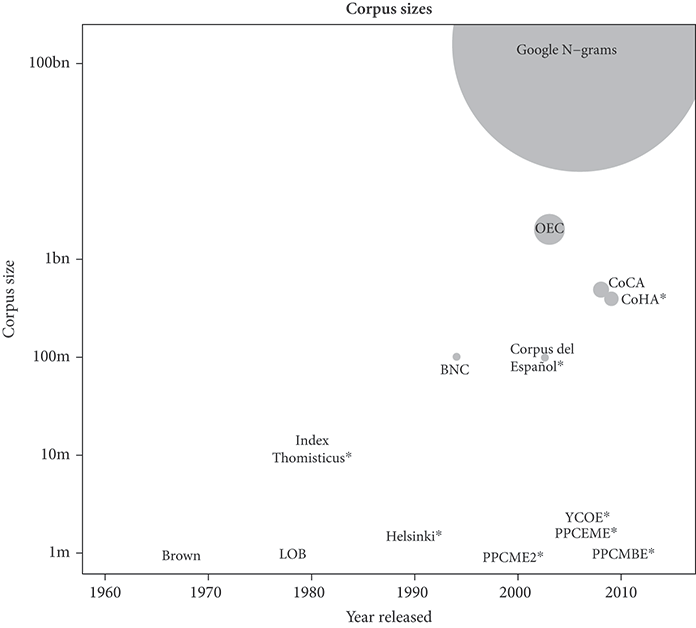
\includegraphics{corpora}
\caption{\label{fig:corpora} Selected historical and modern corpora by year and size, image from \citet{quantitative-historical}.}
\end{figure}

A more prominent and conventional way of utilizing computational methods in historical linguistics, which is simultaneously highly relevant to this thesis, is for quantitative, corpus-based inquiries. As \citet{gillivray_2023} note, corpus-based research and quantitative research in this field has been on the rise in the recent years. \citet{quantitative-historical} also present a framework for working with historical data in a quantitative way. They highlight that these methods are often pioneered by people interested in the new technology that is available and in ways to apply it to historical linguistics. It is therefore difficult to define the field of computational historical linguistics as anything other than the overlap between the methods and tools utilized in a variety of computational fields and historical data. \citet{quantitative-historical} argue strongly in favor of well-annotated corpora, highlighting the importance of not only thorough content annotation, but also the inclusion of metadata. They note that in the case of manual annotation, strict guidelines should be enforced, and mention automated annotation as a promising field - although historical data does present various issues for such an approach, especially when the tools used are not well-adapted.

Another interesting computational approach, implemented by \citet{johannsen-etal-2015-cross}, pertains to assessing variation in syntax. While the authors of this paper focus on the variation between users of a language based on age and gender, this approach could likely be implemented for diachronic studies as well. According to the authors, this method allows for a larger amount of data to be analyzed than traditional sociolinguistic methods. The authors use a state-of-the-art dependency parser to annotate their data and then analyse dependency patterns based on so-called treelets, i.e. pairs of UPOS tags connected by a dependency relation. 

\subsection{Part-of-speech tagging of historical data}
\label{subsec:historical-pos-tagging}

One area that could be said to be balancing between NLP and (computational) historical linguistics is part-of-speech tagging of historical data. Research of this kind is conducted for a variety of reasons: on the one hand, evaluating the way in which taggers adapted to modern data perform on historical data can help improve the tools and pre-processing procedures themselves, and on the other hand, the ability to accurately tag data using automated tools, as mentioned in \autoref{subsec:comp-hist-ling}, is highly relevant for the creation of corpora. 

\begin{table*}[h]
\begin{center}
\begin{tabular}{|l|cccc|}
\hline \bf Paper & \bf Language & \bf \makecell[c]{Tagger Test Set \\ Accuracy (\%)} & \bf \makecell[c]{Historical \\ Test Data \\ Accuracy (\%)} & \bf \makecell[c]{Preprocessed \\ Historical \\ Test Data \\ Accuracy (\%)} \\ \hline
\citet{rayson07} & English & 96 & 82--88.5\% & 89--93.2\% \\
\citet{scheible11} & German & - & 69.6\% & 79.7\% \\
\citet{bollmann-2013-pos} & German & - & 23--81.8\% & 83.4--95.6\% \\
\citet{hupkes16} & Dutch & 96 & 60\% & 92\% \\
\citet{adesam-bouma-2016-old} & Swedish & 94.2\footnotemark & 45\% & 70\% \\
%\citet{waszczuk2018morphosyntactic} & Polish &  - & \makecell[c]{precision and recall: \\ 88.3--90.3\%\\88.3--90.3\%} & - \\
\hline
\end{tabular}
\end{center}
\caption{\label{table:others-tagging-results} Test results on modern, historical and preprocessed historical data in other experiments. Note: these experiments used different kinds of taggers, tagsets, pre-processing methods, and data, which means that their results are not fully comparable.}
\end{table*}
\footnotetext{Here the tagger was trained on historical data as well.}

\autoref{table:others-tagging-results} presents a variety of studies where various taggers, predominantly trained on modern data, were tested on historical data, with and without preprocessing. Not included in the table is \citet{waszczuk2018morphosyntactic}, as the measures that they do not provide accuracy as a measure, but instead use precision and recall (both around 88.3 for baroque texts and 90.3\% for texts from 1830-1918). They also do not utilize any preprocessing procedures. However, this study is highly relevant to the topic of the thesis as not only does it tackle Polish, but also tests one of the taggers tested in the subsequent sections. 

\subsection{Computational background}
\label{subsec:algorithms}

Although their use in this thesis is discussed in more detail in \autoref{sec:exp-setup}, relevant algorithms and architectures are be introduced in this subsection. It is important to note that this thesis does not attempt to improve any of these, but instead tests how they can be utilized in similar inquiries. 

\begin{figure}[H]
\centering
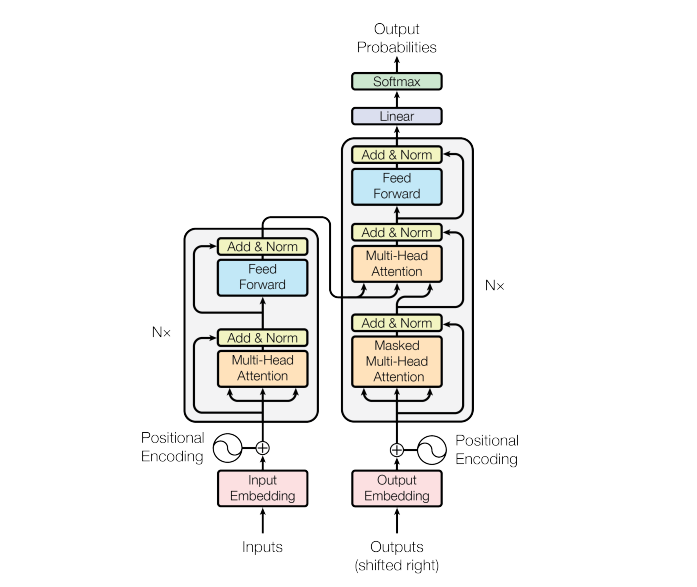
\includegraphics{transformers}
\caption{\label{fig:transformers} The architecture of a transformer model, image from \citet{vaswani2017attention}.}
\end{figure}

Within this thesis, a selection of pre-trained tools are used. These include \cite{waszczuk-2012-harnessing} and \citet{kie:wol:17:morf}'s Morfeusz2 and Concraft-pl, \citet{qi2020stanza}'s Stanza neural pipeline, and \citet{gatecloud}'s UPOS tagger. In addition, two pre-existing tagger architectures are trained on selected data. These include a pipeline provided by \citet{wolf-etal-2020-transformers} for utilizing any of the HuggingFace BERT-like models (in the case of this thesis it was \citet{kłeczek_2021}'s BERT for Polish). These harness the power of the so-called transformer neural model architecture (as depicted in \autoref{fig:transformers}), first introduced by \citet{vaswani2017attention}, which employs attention to determine which elements should weigh in on the result; this allows the model to better take into account which elements of the sentence can indicate the appropriate tag, in addition to the information from the word representation. The other trainable tagger architecture is Marmot, an improved Conditional Random Fields-based tagger, using what authors call "pruned CRFs." This approach consists of "[creating] increasingly complex lattices and to [filtering] candidate states at every step to prevent a polynomial increase in lattice size" \citep{mueller-etal-2013-efficient}. The method for this is presented in \autoref{fig:marmot}. 

\begin{figure}[H]
\centering
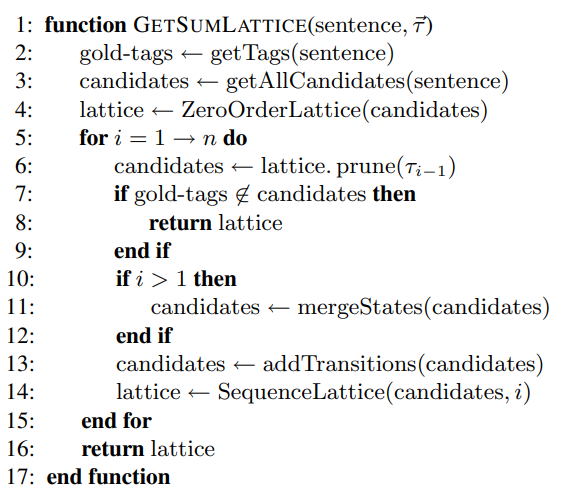
\includegraphics[scale=0.6]{marmot}
\caption{\label{fig:marmot} A mock-algorithm for CRF pruning, image from \citet{mueller-etal-2013-efficient}.}
\end{figure}

In addition, this thesis makes use of a number of existing libraries for Python 3 and their implementations of various algorithms and measures, such as the evaluation measure calculations provided by \citet{scikit-learn} or \citet{reback2020pandas}'s data structures. 







